\chapter{Discussion}\label{chap:discussion}

We have already reviewed the main research themes around quantum compilation in Chapter~\ref{chap:background}. We have seen that one of the main challenges is in imposing connectivity constraints on the circuit. Furthermore, because of the huge dependence of most of the research on swapping qubits, along with the fact that swapping is the most expensive two-qubit gate, it is important to study the alternatives for swapping. In this chapter, we introduce our research problem based on the definition of bridging that we discussed earlier.

\section{Problem Statement}

While our aim in the broadest term is to find alternatives to the SWAP gate to apply gates with respect to connectivity constraints, we start with a more specific problem. We seek the optimal bridged gate, and by optimal we mean both the least number of CNOTs and the least depth. Note that, this problem is going to be studied for an arbitrary connectivity constraint $G$.

The relation of this problem to the approach of \cite{nash2020,kissinger2019} is that we are looking for bridged gates that can be adopted in any compilation process, in contrast to theirs that defines a whole new compilation process. In terms of the results, while some of our preliminary results such as a simple bridged CNOT gate can be derived from their techniques too, however, the main contribution of our work is to show the optimal bridged gate for any two-qubit gate, while those efforts are limited to compiling the gates that are combinations of CNOTs and $R_z$s.

\section{Two-qubit Gate Classes}

Our discussion heavily relies on the KAK decomposition of two-qubit gates. We have already introduced it in Lemma~\ref{lem:kak_decomposition}. Here we introduce a few classes of two-qubit gates, based on their KAK decomposition.

\begin{definition}[Two-qubit Gate Classes]
  Based on the KAK decomposition of two-qubit gates, that is
  \begin{equation}
    U = (V_1 \otimes V_2) e^{i \alpha X \otimes X + i \beta Y \otimes Y + i \gamma Z \otimes Z} (V_3 \otimes V_4),
  \end{equation}
  we define the following classes of two-qubit gates:
  \begin{itemize}
    \item \textbf{Class nil}: Two-qubit gates that $\alpha = \beta = \gamma = 0$.
    \item \textbf{Class I:} Two-qubit gates that only one of $\alpha, \beta, \gamma \neq 0$.
    \item \textbf{Class II:} Two-qubit gates that at least two of $\alpha, \beta, \gamma \neq 0$.
  \end{itemize}
\end{definition}

The gates in class nil are local gates that are applied on each qubit separately, so they are irrelevant to our discussion about bridging. The gates in class I, such as CNOT, CZ and etc., can be decomposed to one $\mathrm{C}R_x$ gate upto local gates. This fact is shown in Lemma~\ref{lem:crx-decomposition} and enables us to bridge them.

\begin{lemma}\label{lem:crx-decomposition}
  For any two-qubit gate $U$ in class I, it can be decomposed as
  \begin{equation}
    U = W_1 \otimes W_2 \mathrm{C}R_x(\theta) W_3 \otimes W_4,
  \end{equation}
  where $\mathrm{C}R_x(\theta)$ is a controlled rotation gate around $x$ axis, with control on the first qubit and target on the second qubit.
\end{lemma}
\begin{proof}
  Without losing generality, we can assume that $\gamma \neq 0$ and $\alpha = \alpha = 0$. Now, we can write
  \begin{equation}
    U = (V_1 \otimes V_2) e^{i \gamma Z \otimes Z} (V_3 \otimes V_4).
  \end{equation}
  Then, similar to the way that we derive $\mathrm{C}Z$ and $\mathrm{CNOT}$ gates, we can write
  \begin{equation}
    \begin{aligned}
    U &= (V_1 \otimes V_2 R_z(-2\gamma)) CR_z(4\theta) (V_3 \otimes V_4), \\
    &= (V_1 \otimes V_2 R_z(-2\gamma) H) CR_x(4\theta) (V_3 \otimes H V_4).
    \end{aligned}
  \end{equation}
  Now $W_i$s are easily derived from $V_i$s.
\end{proof}

The gates in class II, such as SWAP, cannot be bridged any better than the baseline implementation mentioned in Corollary~\ref{cor:baseline-bridged}. This fact is shown later using an special trait of these gates in Lemma~\ref{lem:no-trivial-commutation}.

\section{Bridged Gates}

Here we introduce the bridged $T$ gate for any $T$ that belongs to class I. This gate is shown under a linear connectivity constraint, so it can be used for any other connectivity constraint (by using the connecting path between the qubits). An example of this gate (bridging over $4$ qubits) is shown in Figure~\ref{fig:bridged-class-i}. Note that $V_i$s and $\theta$ can be computed using Lemma~\ref{lem:crx-decomposition}

\begin{figure}[h!]
  \label{fig:bridged-class-i}
  \centering
  \begin{tikzpicture}
    \node[scale=0.7] {
\begin{quantikz}[transparent]
  \qw &\gate[6]{T}                        &\qw\midstick[6,brackets=none]{=}&
  \qw &\gate{V_3} & \ctrl{5} & \gate{V_1} &\qw\midstick[6,brackets=none]{=}&
  \gate{V_3} & \targ{}  & \qw     &\ctrl{1}& \qw    & \qw    & \qw    &\ctrl{1}& \qw     &\targ{}&\gate{V_1}\\
  \qw &\linethrough &\qw &
  \qw &\qw &\qw &\qw &\qw &
  \qw & \ctrl{-1}&\targ{}  & \targ{}&\ctrl{1}& \qw    &\ctrl{1}&\targ{} &\targ{}  &\ctrl{-1}&\qw\\
  \qw &\linethrough &\qw &
  \qw &\qw &\qw &\qw &\qw &
  \qw & \qw &\ctrl{-1}& \qw    & \targ{}&\ctrl{1}&\targ{} & \qw    &\ctrl{-1}&\qw & \qw \\
  \qw &\linethrough &\qw &
  \qw &\qw &\qw &\qw &\qw &
  \qw & \qw &\targ{}  & \qw    &\ctrl{1}& \gate{R_x(\theta)}&\ctrl{1}& \qw    &\targ{}  &\qw & \qw\\
  \qw &\linethrough &\qw &
  \qw &\qw &\qw &\qw &\qw &
  \qw & \targ{}  &\ctrl{-1}&\ctrl{1}& \targ{}& \qw    &\targ{} &\ctrl{1}&\ctrl{-1}&\targ{}&\qw \\
  \qw &  & \qw &
  \qw &\gate{V_4} & \gate{R_x(\theta)} & \gate{V_2} & \qw&
  \gate{V_4} & \ctrl{-1}& \qw     & \targ{}& \qw    & \qw    & \qw    &\targ{} & \qw     &\ctrl{-1}& \gate{V_2} 
  \end{quantikz}
  };
  \end{tikzpicture}
  \caption{A bridged class I gate over 6 qubits}
\end{figure}
  
This circuit above can be mathematically defined as follows:

\begin{proposition}[Bridged class I gate]\label{prop:bridged-class-i}
  For any class I two-qubit gate $T$, A bridged $T$ gate defined on qubits $1, n \in V$, where every $(i, i + 1) \in E$, can be implemented by the following sequence of gates:
  \begin{equation}
    T = (V_1 \otimes V_2) B^\dagger_n \mathrm{C}R_x^{\lceil n/2 \rceil \to \lceil n/2\rceil+1}(\theta) B_n (V_3 \otimes V_4),
  \end{equation}
  where $V_i$s and $\theta$ are defined in Lemma~\ref{lem:crx-decomposition}, and $B_n$ for $n = 4$ is defined as follows:
  \begin{equation}
    B_4 = (\CNOT^{1 \to 2} \otimes \CNOT^{3 \to 4}) (\CNOT^{2 \to 1} \otimes \CNOT^{4 \to 3}),
  \end{equation}
  and for an even $n \ge 6$ it could be written as follows:
  \begin{equation}
    \begin{aligned}
    B_{n} = &(\CNOT^{n/2 - 1 \to n/2} \otimes \CNOT^{n/2 + 1 \to n/2 + 2}) \\
    &(\CNOT^{n/2 - 2 \to n/2 - 1} \otimes \CNOT^{n/2 + 2 \to n/2 + 3}) \\
    &\prod_{i=1}^{n/2 - 3} (\CNOT^{i \to i+1} \otimes \CNOT^{i+3 \to i+2} \otimes \CNOT^{n-i-1 \to n-i-2} \otimes \CNOT^{n-i \to n-i+1}) \\
    &(\CNOT^{3 \to 2} \otimes \CNOT^{n-1 \to n-2}) \\
    &(\CNOT^{2 \to 1} \otimes \CNOT^{n \to n-1}).
    \end{aligned}
  \end{equation}
  and, for any odd $n$ it could be recovered by removing $n$th qubit and its corresponding CNOTs from $B_n$.
\end{proposition}
\begin{proof}
  In order to prove the correctness of this circuit, we will show that it is equivalent to the baseline implementation of the bridged $T$ gate (Corollary~\ref{cor:baseline-bridged}).
  
  First, using the fact that $[\CNOT^{i \to j}, \CNOT{i \to k}] = 0$ and $[\CNOT^{i \to j}, \CNOT^{k \to j}] = 0$, we can show that $B_n$ (for even $n$) could be rearranged as:

  \begin{equation}
    B_n = \prod_{i=1}^{n/2 - 1} (\CNOT^{i\to i+1}\CNOT{i+1\to i}) \otimes (\CNOT^{n-i\to n-i+1} \CNOT{n-i+1\to n-i}).
  \end{equation}

  This rearrangement for $n = 6$ is shown in Figure~\ref{fig:bridged-class-i-proof-a}.

  \begin{figure}[h!]
    \label{fig:bridged-class-i-proof-a}
    \centering
    \begin{tikzpicture}
      \node[scale=0.6] {
  \begin{quantikz}[transparent]
    \gate{V_3} & \targ{}  & \qw     &\ctrl{1}& \qw    & \qw    & \qw    &\ctrl{1}& \qw     &\targ{}&\gate{V_1}&\qw\midstick[6,brackets=none]{=}&
    \gate{V_3} & \targ{}  &\ctrl{1}& \qw     & \qw    & \qw    & \qw    & \qw     &\ctrl{1}&\targ{}&\gate{V_1}& \qw \\
    \qw & \ctrl{-1}&\targ{}  & \targ{}&\ctrl{1}& \qw    &\ctrl{1}&\targ{} &\targ{}  &\ctrl{-1}&\qw&\qw&
    \qw & \ctrl{-1}&\targ{}  & \targ{}&\ctrl{1}& \qw    &\ctrl{1}&\targ{} &\targ{}  &\ctrl{-1}&\qw&\qw\\
    \qw & \qw &\ctrl{-1}& \qw    & \targ{}&\ctrl{1}&\targ{} & \qw    &\ctrl{-1}&\qw & \qw & \qw &
    \qw & \qw & \qw    &\ctrl{-1}& \targ{}&\ctrl{1}&\targ{} &\ctrl{-1}& \qw    &\qw & \qw & \qw \\
    \qw & \qw &\targ{}  & \qw    &\ctrl{1}& \gate{R_x(\theta)}&\ctrl{1}& \qw    &\targ{}  &\qw & \qw&\qw&
    \qw & \qw   & \qw    &\targ{}&\ctrl{1}& \gate{R_x(\theta)}&\ctrl{1}&\targ{}& \qw      &\qw & \qw&\qw&\\
    \qw & \targ{}  &\ctrl{-1}&\ctrl{1}& \targ{}& \qw    &\targ{} &\ctrl{1}&\ctrl{-1}&\targ{}&\qw&\qw& 
    \qw & \targ{}  &\ctrl{1}&\ctrl{-1}& \targ{}& \qw    &\targ{} &\ctrl{-1}&\ctrl{1}&\targ{}&\qw&\qw\\
    \gate{V_4} & \ctrl{-1}& \qw     & \targ{}& \qw    & \qw    & \qw    &\targ{} & \qw     &\ctrl{-1}& \gate{V_2} &\qw&
    \gate{V_4} & \ctrl{-1}& \targ{} & \qw  & \qw    & \qw    & \qw     & \qw     &\targ{}&\ctrl{-1}& \gate{V_2} &\qw&
    \end{quantikz}
    };
    \end{tikzpicture}
    \caption{Rearrangement of CNOTs that is used in the proof}
  \end{figure}

  Then, using the fact that 
  \begin{equation}
    \SWAP^{i,j} = \CNOT^{j \to i} \CNOT^{i \to j} \CNOT^{j \to i},
  \end{equation}
  it could be simplified further to
  \begin{equation}
    B_n = \prod_{i=1}^{n/2 - 1} (\CNOT^{i+1 \to i} \SWAP^{i, i+1}) \otimes (\CNOT{n-i+1\to n-i}\SWAP^{n-i, n-i+1}).
  \end{equation}

  Now, by moving the rearranging the CNOTs to be applied after the SWAPs, we will have
  \begin{equation}
    B_n = \prod_{i=1}^{n/2 - 1} \CNOT^{n/2 \to i} \otimes \CNOT^{n-i+1 \to n/2 + 1} \prod_{i=1}^{n/2 - 1} \SWAP^{i, i+1} \otimes \SWAP^{n-i, n-i+1}.
  \end{equation}

  This process is shown in Figure~\ref{fig:bridged-class-i-proof-b} for $n = 6$.
  
  \begin{figure}[h!]
    \label{fig:bridged-class-i-proof-b}
    \centering
    \begin{tikzpicture}
      \node[scale=0.6] {
  \begin{quantikz}[transparent]
    \gate{V_3} & \swap{}  &\targ{}& \qw     & \qw    & \qw    & \qw    & \qw     &\targ{}&\swap{}&\gate{V_1}&\qw\midstick[6,brackets=none]{=}&
    \gate{V_3} & \swap{}  & \qw     &\targ{}& \qw    & \qw    & \qw    &\targ{}& \qw     &\swap{}&\gate{V_1}&\qw \\
    \qw & \swap{-1}&\ctrl{-1}  & \swap{}&\targ{}& \qw    &\targ{}&\swap{} &\ctrl{-1}  &\swap{-1}&\qw&\qw&
    \qw & \swap{-1}& \swap{}&\qw&\targ{}& \qw    &\targ{}&\qw &\swap{} &\swap{-1}&\qw&\qw\\
    \qw & \qw & \qw    &\swap{-1}& \ctrl{-1}&\ctrl{1}&\ctrl{-1} &\swap{-1}& \qw    &\qw & \qw & \qw &
    \qw & \qw &\swap{-1}& \ctrl{-2} & \ctrl{-1}&\ctrl{1}&\ctrl{-1} &\ctrl{-2}& \swap{-1}    &\qw & \qw & \qw\\
    \qw & \qw   & \qw    &\swap{1}&\targ{}& \gate{R_x(\theta)}&\targ{}&\swap{1}& \qw      &\qw & \qw&\qw&
    \qw & \qw   & \swap{1}    &\targ{}&\targ{}& \gate{R_x(\theta)}&\targ{}&\targ{}& \swap{1}      &\qw & \qw&\qw\\
    \qw & \swap{1}  &\targ{}&\swap{}& \ctrl{-1}& \qw    &\ctrl{-1} &\swap{}&\targ{}&\swap{1}&\qw&\qw& 
    \qw & \swap{1}  &\swap{}&\qw& \ctrl{-1}& \qw    &\ctrl{-1} &\qw&\swap{}&\swap{1}&\qw&\qw\\
    \gate{V_4} & \swap{}& \ctrl{-1} & \qw  & \qw    & \qw    & \qw     & \qw     &\ctrl{-1}&\swap{}& \gate{V_2} &\qw&
    \gate{V_4} & \swap{}&  \qw & \ctrl{-2} & \qw    & \qw    & \qw     &\ctrl{-2}& \qw     &\swap{}& \gate{V_2} &\qw
    \end{quantikz}
    };
    \end{tikzpicture}
    \caption{Moving CNOTs across the SWAPs that is used in the proof}
  \end{figure}

  Finally, the second product term is similar to the one in Corollary~\ref{cor:baseline-bridged}, and the first product term is a sequence of CNOTs that all commute with $\mathrm{C}R_x^{n/2 \to n/2 + 1}(\theta)$, so they will be canceled in $B_n^\dagger \mathrm{C}R_x^{n/2 \to n/2 + 1}(\theta) B_n$.

  \begin{equation}
    \begin{aligned}
    B^\dagger_n \mathrm{C}R_x^{n/2 \to n/2 + 1}(\theta) B_n &= \prod_{i=n/2 - 1}^{1} \SWAP^{i, i+1} \otimes \SWAP^{n-i, n-i+1} \\
    & \phantom{=}~\mathrm{C}R_x^{n/2 \to n/2 + 1}(\theta) \\
    & \phantom{=}~\prod_{i=1}^{n/2 - 1} \SWAP^{i, i+1} \otimes \SWAP^{n-i, n-i+1} \\
    &= \mathrm{C}R_x^{1 \to n}(\theta).
    \end{aligned}
  \end{equation}

  Finally, by recalling Lemma~\ref{lem:crx-decomposition},
  \begin{equation}
    (V_1 \otimes V_2) B^\dagger_n \mathrm{C}R_x^{\lceil n/2 \rceil \to \lceil n/2\rceil+1}(\theta) B_n (V_3 \otimes V_4) = T.
  \end{equation}
  
  In order to prove the correctness of the circuit for odd $n$ as well, we can simply remove the $n$th qubit and its corresponding CNOTs from $B_n$. This fact will be propagated through the proof and every other thing will be the same.
\end{proof}

The formula above shows that the circuit uses $4n + O(1)$ CNOTs with the depth $n + O(1)$ (noting that $\mathrm{C}R_x$ needs two CNOTs \cite[chapter 4]{nielsen2010}).
While in comparison to the baseline implementation (see Corollary~\ref{cor:baseline-bridged}), this circuit has $33\%$ improvement in the number of CNOTs and $66\%$ improvement in the depth. Even for the special case of CNOT, this circuit has approximately the same number of CNOTs as the bridged CNOT gate in Equation~\ref{eq:bridged-cnot-m-n} and Figure~\ref{fig:bridged-cnot-m-n}, however, its depth is improved by $75\%$.

\section{Proof of Optimality}

Now, we aim to prove the optimality of the bridged $T$ gate described in the previous section for class I gates, and the baseline implementation for class II gates. By optimality we mean that the number of CNOTs and the depth of the circuit is the minimum possible (upto an $O(1)$ constant).

Here we first introduce the tools and the intuition behind their definitions, in addition to the core lemma that is used in the proofs. Then, we will prove a general lower bound for the depth, followed by the lower bounds for the number of CNOTs for class I and class II gates separately. Starting by the first tool that we need is conjugation that is commonly used in group theory \cite{weisstein}.

\begin{definition}[Conjugation]
  For any two gates $A$ and $B$, we define the conjugation of $A$ by $B$ as
  \begin{equation}
    B^\dagger A B.
  \end{equation}
\end{definition}

The intuition behind the conjugation of gates is that if the conjugation of $A$ by $B$ is $C$, then applying $A$ before $A$ is equivalent to applying $C$ after $B$. Informally this could be phrased as by crossing $A$ over $B$, $A$ will be transformed to $C$. Figure~\ref{fig:conjugations} shows a few conjugations that we will use in the proofs.

\begin{figure}[h!]\label{fig:conjugations}
  \centering
  \begin{tikzpicture}
    \node at (-3, 0.4) {a)};
    \node[scale=0.7] {\begin{quantikz}
    \qw & \gate{X} & \ctrl{1} & \qw\midstick[2,brackets=none]{=} & \qw & \ctrl{1} & \gate[2]{U} & \qw \\
    \qw & \qw & \gate{R_x} & \qw & \qw & \gate{R_x} & \qw & \qw 
  \end{quantikz}};\end{tikzpicture} \\
  \begin{tikzpicture}
    \node at (-3, 0.4) {b)};
    \node[scale=0.7] {\begin{quantikz}
    \qw & \gate{Z} & \ctrl{1} & \qw\midstick[2,brackets=none]{=} & \qw & \ctrl{1} & \gate{Z} & \qw \\
    \qw & \qw & \gate{R_x} &  & \qw & \gate{R_x} & \qw & \qw 
  \end{quantikz}};\end{tikzpicture} \\
  \begin{tikzpicture}
    \node at (-3, 0.4) {c)};
    \node[scale=0.7] {\begin{quantikz}
    \qw & \gate{U} & \swap{1} & \qw\midstick[2,brackets=none]{=} & \qw & \swap{1} & \qw &  \qw \\
    \qw & \qw & \swap{} & \qw & \qw & \swap{} & \gate{U} & \qw 
  \end{quantikz}};\end{tikzpicture}
  \caption{a) Conjugation of $X \otimes I$ by $\mathrm{C}R_x$ is a two-qubit gate. b) The conjugation of $Z \otimes I$ by $\mathrm{C}R_x$ is $Z \otimes I$. c) The conjugation of $U \otimes I$ by SWAP is $I \otimes U$.}
\end{figure}

Furthermore, this effect will help us to develop a tool to properly analyse the flow of information in a circuit. To complete this idea we define a sense of locality, using the following simple definition:

\begin{definition}[Trivial/Nontrivial action]
  A gate $U$ defined on a set of qubits $Q$ is acting trivially on qubit $q \in Q$ if $U$ can be written as 
  \begin{equation}
    U = U' \otimes I_q
  \end{equation}
  where $U'$ is a gate defined on $Q \setminus \{ q \}$ and $I_q$ is the identity gate on qubit $q$.
  Respectively, $U$ is acting nontrivially on $q$ if it cannot be written in the above form.
\end{definition}

Now, these proofs are based on the idea that if two gate sequences $A = A_n \dots A_2 A_1$ and $B = B_m \dots B_2 B_1$ are equal, then the conjugation of any arbitrary gate $U$ by $A$ is equal to the conjugation of $U$ by $B$. Or in another word,

\begin{corollary}
  Assume $A = A_n \dots A_2 A_1$ and $B = B_m \dots B_2 B_1$ are two gate sequences, then the necessary condition for $A = B$ is that for any arbitrary gate $U$, the conjugation of $U$ by $A$ must be equal to the conjugation of $U$ by $B$.
\end{corollary}

This corollary will be of incredible useful if one notices that the conjugation of $U$ by $A$ can be computed iteratively as follows:

\begin{equation}
  \begin{cases}
    U_1 = \text{conjugation of } U \text{ by } A_1 \\
    U_{i+1} = \text{conjugation of } U_i \text{ by } A_{i+1}
  \end{cases}
  \Rightarrow U_n = \text{conjugation of } U \text{ by } A.
\end{equation}

Now, here present a set of facts that use definiton of trivial/nontrivial action to specify the conjugation of gates by each class of gates.

\begin{corollary}[No-go for one-qubit gates]\label{cor:no-go-one-qubit}
  For any gate acting trivially on $t$, its conjugation by any one-qubit gate on $t$ is still trivial on $t$. 
\end{corollary}

This corollary informally states that if we want to create nontrivial action on $t$ by conjugation, we need use two-qubit gates. This fact can be easily shown by simply combining definition of trivial action and conjugation.

Then, we independently prove the following lemma for class I gates, that informally states a single class I gate, cannot move nontrivial action (creating on one qubit and destroying on another).

\begin{lemma}[No move for class I]\label{lem:no-move-class-i}
  For any gate $A$ acting nontrivially on $n$ and trivially on $t$, its conjugation $B$ by any class I gate $U$ acting on $n$ and $t$, is nontrivial on $n$.
\end{lemma}
\begin{proof}
  Noting that $A$ must be trivial on $t$ and nontrivial on $n$, $A$ could be decomposed as $A' \otimes I_t$.
  Using the definition of conjugation in form of $U^\dagger A U = B$, we can write

  \begin{equation}
    \begin{aligned}
    B &= U^\dagger (A' \otimes I_t) U  \\
    &= (V_3^\dagger \otimes V_4^\dagger)\mathrm{C}R_x(-\theta) (V_1^\dagger A' V_1 \otimes I) \mathrm{C}R_x(\theta) (V_3 \otimes V_4) \\
    &= (V_3^\dagger \otimes V_4^\dagger)(\dyad{0} + R_x(-\theta) \otimes \dyad{1}) (V_1^\dagger A' V_1 \otimes I) (\dyad{0} + R_x(\theta) \otimes \dyad{1}) (V_3 \otimes V_4) \\
    &= (V_3^\dagger \otimes V_4^\dagger)(V_1^\dagger A' V_1 \dyad{0} + R_x(-\theta) V_1^\dagger A' V_1 R_x(\theta) \dyad{1}) (V_3 \otimes V_4)
    \end{aligned}
  \end{equation}

  We have used the decomposition of Lemma~\ref{lem:crx-decomposition} for $U$ and expanded $\mathrm{C}R_x$ in terms of $\dyad{0}$ and $\dyad{1}$. Then, in order to proof by contradiction, we can assume that $B = I_n \otimes B'$, then $\tr_n(B) = B'$, so
  \begin{equation}
    B' = \tr_n(B) = \tr_n(A') \dyad{0}_n + \tr_n(A') \dyad{1}_n = \tr_n(A') I_t
  \end{equation}
  which means that $B = \tr_n(A') \otimes I_n \otimes I_t$, that results in $A = \tr_n(A') \otimes I_n \otimes I_t$. This contradicts the assumption that $A$ is not trivial in $n$.
\end{proof}

Afterward, by using a similar approach, we can prove that there is no gate can stay on just one of the qubits after conjugation by a class II gate, while this fact is not true for class I gates and has been shown in Figure~\ref{fig:conjugations}.

\begin{lemma}[No stationary for class II]\label{lem:no-trivial-commutation}
  For any gate $A$ that acts nontrivially on $n$ and trivially on $t$, its conjugation $B$ by a class II gate $U$ acting on $n$ and $t$, is nontrivial on $t$. 
\end{lemma}
\begin{proof}
  Similar to the approach in proving Lemma~\ref{lem:no-move-class-i}, using proof by contradiction, we can assume that $B = B' \otimes I_t$, then
  \begin{equation}
    \begin{aligned}
      (A' \otimes I_t) U  &= U (B' \otimes I_t) \\
      (A' V_1 \otimes V_2) e^{i \alpha X \otimes X + i \beta Y \otimes Y + i \gamma Z \otimes Z} (V_3 \otimes V_4) &= (V_1 \otimes V_2) e^{i \alpha X \otimes X + i \beta Y \otimes Y + i \gamma Z \otimes Z} (V_3 B' \otimes V_4). 
    \end{aligned}
  \end{equation}
  Then by multiplying $(V_1^\dagger \otimes V_2^\dagger)$ from left and $(V_3^\dagger \otimes V_4^\dagger)$ from right, we can write
  \begin{equation}
      (V_1^\dagger A' V_1 \otimes I_t) e^{i \alpha X \otimes X + i \beta Y \otimes Y + i \gamma Z \otimes Z} = e^{i \alpha X \otimes X + i \beta Y \otimes Y + i \gamma Z \otimes Z} (V_3 B' V_3^\dagger \otimes I_t).
  \end{equation}

  Now, by expanding the exponential, we will have
  \begin{equation}
    \begin{aligned}
      (V_1^\dagger A' V_1 \otimes I_t) & (c_1 I \otimes I + i c_2 X \otimes X + i c_3 Y \otimes Y + i c_4 Z \otimes Z) \\
      = &(c_1 I \otimes I + i c_2 X \otimes X + i c_3 Y \otimes Y + i c_4 Z \otimes Z) (V_3 B' V_3^\dagger \otimes I_t).  
    \end{aligned}
  \end{equation}
  Where $c_i$s are some constants. Finally, by multiplying both sides by $(I_n \otimes P)$ where $P$ is one of $I, X, Y, Z$, and then by tracing out the qubit $t$, we will have the following equations:
  \begin{equation}
    \begin{cases}
      V_1^\dagger A' V_1 = V_3 B' V_3^\dagger \\
      V_1^\dagger A' V_1 X = X V_3 B' V_3^\dagger & \text{if }\alpha \ne 0 \\
      V_1^\dagger A' V_1 Y = Y V_3 B' V_3^\dagger & \text{if }\beta \ne 0 \\
      V_1^\dagger A' V_1 Z = Z V_3 B' V_3^\dagger & \text{if }\gamma \ne 0. \\
    \end{cases}
  \end{equation}

  It means that if two of $\alpha, \beta, \gamma$ are non-zero, then $A$ must have the form $A' = A'' \otimes I_n$ which is against the assumption that $A$ is nontrivial on $n$.
\end{proof}

Finally, using the previous lemma, we can prove a less restrictive claim for both classes I and II, that states that there is always a gate that will not stay on its qubit after conjugation.

\begin{lemma}[Nonstationary for classes I and II]\label{lem:nontrivial-commutation}
    For an arbitrary two-qubit gate $T$ that is not a class nil gate and is defined on qubits $a$ and $b$, there exists one-qubit gate $U$ defined on $a$ that the conjugation of $U$ under $T$ acts nontrivially on $b$.
\end{lemma}
\begin{proof}
    For class I, if we use Lemma~\ref{lem:crx-decomposition} and the fact that the conjugation of a gate is a bijective function of that gate, then the problem reduces to the existence of such $U$ for $T = \mathrm{C}R_x^{a\to b}(\theta)$, which is trivially true by choosing $U = X$.

    For class II, this is the direct result of Lemma~\ref{lem:no-trivial-commutation}.
\end{proof}

Now, for the first result we can prove the minimum necessary depth for bridging any two-qubit gate that does not belong to class nil.

\begin{proposition}\label{prop:no-go-depth}
    Any bridged $T$ gate where $T$ is not a class nil gate and acts on qubits $1$ and $n$, and bridging is done with a linear connectivity constraint, the bridged gate has at least $n + O(1)$ depth.
\end{proposition}
\begin{proof}
  Using Lemma~\ref{lem:nontrivial-commutation}, there exists a $U$ defined on qubit $1$ where the conjugation of $U$ by $T$ acts nontrivially on qubit $n$. Now, if the bridged $T$ gate is implemented by the gate sequence $A = A_\ell \dots A_2 A_1$, then the conjugation of $U$ by $A$ is nontrivial on $n$. 

  We name the conjugation of $U$ by $A_j \dots A_2 A_1$ as $u_j$, and we want $u_\ell$ to be nontrivial on $n$. We know that the gates that can be applied on $n$ are one-qubit gates and $\CNOT^{n-1\rightleftharpoons n}$. Corollary~\ref{cor:no-go-one-qubit} states that one-qubit gates could not introduce nontrivial action in this case, so the only way is to apply $\CNOT^{n-1\rightleftharpoons n}$ at some point, which means that
  \begin{equation}
    A_j = \CNOT^{n-1\rightleftharpoons n} \otimes A'_{j} \text{ for some } j.
  \end{equation}
  By $\CNOT^{a \rightleftharpoons b}$ we mean the CNOT gate that can have arbitrary direction. Then, note that if $u_{j-1}$ acts trivially on $n-1$, it would not be possible to make $u_j$ nontrivial on $n$, therefore we can conclude that $u_{j-1}$ acts nontrivially on $n-1$. 

  Now, we can repeat the same argument for $n-1$ and $u_{j-1}$, and we can conclude that
  \begin{equation} 
    A_k = \CNOT^{n-2\rightleftharpoons n-1} \otimes A'_{k} \text{ for some } k < j,
  \end{equation}
  and $u_{k-1}$ acts nontrivially on $n-2$. Continuing this argument, we can find $c_{n-1}, \dots c_1$ such that $c_i < c_{i+1}$ and
  \begin{equation}
    A_{c_i} = \CNOT^{i\rightleftharpoons i+1} \otimes A'_{c_i},
  \end{equation}
  and $u_{c_i-1}$ acts nontrivially on $i$.
  The existence of $c_i$ gauranties that the depth of the circuit is at least $n-1$.
\end{proof}

This lower bound is tight for class I gates, as the introduced bridged $T$ gate for class I gates has the same depth. However, for class II gates, this lower bound might not be tight. Next, we will prove separate results for each class.

\subsection{Class I}

The sketch of this proof consists of first reducing the problem to bridging a $\mathrm{C}R_x^{1\to n}$ gate. Then because of the nontrivial (on $1$ and $n$) conjugations of $X_1$ and $Z_n$ by $\mathrm{C}R_x^{1\to n}$, we can conclude that any sequence of gates that is bridged $\mathrm{C}R_x^{1\to n}$ needs to have a minimum number of CNOTs, and a minimum depth, to produce such nontrivial conjugations. These two bounds are achieved by the bridged $T$ gate.

Now, we can prove the optimality of the bridged $T$ gate for class I gates in the following theorem.

\begin{theorem}\label{thm:no-go-class-i}
  Any bridged $T$ gate where $T$ is a class I gate that acts on qubits $1$ and $n$ with linear connectivity, needs at least $4n + O(1)$ CNOTs.
\end{theorem}
\begin{proof}
  Without losing generality, we can assume that $T = \mathrm{C}R_x^{1\to n}(\theta)$, because of Lemma~\ref{lem:crx-decomposition}. We can also show that the conjugation of $X_1$ and $Z_n$ (one-qubit gates acting on qubits $1$ and $n$ respectively) by $T$ is nontrivial on $1$ and $n$. Then we assume that a sequence of gates $A = A_\ell \dots A_2 A_1$ is equivalent to $T$, the conjugation of $X_1$ and $Z_n$ under $A$ must also be nontrivial on $1$ and $n$ as well. In order to simplify the notation, we name the conjugation of $X_1$ and $Z_n$ by $A_i \dots A_1$ as $\xi_i$ and $\zeta_i$ respectively. 
  
  Now, based on the fact that one-qubit gates could not create nontrivial action (Corollary~\ref{cor:no-go-one-qubit}), and because of the connectivity constraint, in order to have nontrivial action on $n$ by $\xi_n$, we need a CNOT gate acting on $n$ and $n-1$, or in other words
  \begin{equation}
    A_j = \CNOT^{n-1\rightleftharpoons n} \otimes A'_{j} \text{ for some } j.
  \end{equation}
  Also $\xi_{j - 1}$, must act nontrivially on $n-1$. Moreover, using Lemma~\ref{lem:no-move-class-i} we know that using one CNOT ($A_j$) will leave $\xi_{j}$ acting nontrivially on $n-1$, which is not desired. This means that at least two CNOTs are necessary, so 
  \begin{equation}
    A_k = \CNOT^{n-1 \rightleftharpoons n-1 \pm 1} \otimes A'_{k} \text{ for some } j < k.
  \end{equation}
  Similarly $\xi_{k-1}$ must act nontrivially on $n-1 \pm 1$.
  
  By recursively applying this argument, we can conclude that a sequence of CNOT pairs acting on subsequent qubits from $1$ to $n$ is necessary solely to make $\xi_n$ have nontrivial action on $n$. A similar argument could hold for $\zeta_n$. Now because of the fact that these two sequences are going in opposite directions, and they cannot have more than $O(1)$ gates in common, we can conclude that at least $4(n-1) + O(1)$ CNOTs are necessary to have nontrivial action on $1$ and $n$ by $\xi_n$ and $\zeta_n$.
\end{proof}

\subsection{Class II}

For the class II, we will prove in a similar way to class I that there is no solution better (in terms of number of CNOTs) than the baseline implementation (Corollary~\ref{cor:baseline-bridged}). 
Now, we can prove the main theorem for class II which states a lower bound for the CNOT count.

\begin{theorem}\label{thm:no-go-class-ii}
  Any bridged gate where $T$ is a class II gate acting on qubits $1$ and $n$ with linear connectivity, needs at least $6n + O(1)$ CNOTs.
\end{theorem}
\begin{proof}
  This proof shares some of its core ideas with the proof of Theorem~\ref{thm:no-go-class-i}.
  Assume that $A_j = \CNOT^{1 \to 2}$ is the only CNOT applying on qubits $1$ and $2$. We have assumed the direction without losing generality as the other direction can be converted by local operations. Now, the conjugation of $Z_1$ (acting on qubit $1$) by $A^\dagger_1 \dots A^\dagger_{j-1}$ that we call $U_1$ must be nontrivial on qubit $1$ and trivial everywhere else. Using Lemma~\ref{lem:no-trivial-commutation}, the conjugation of $U_1$ by $T$ must act nontrivial on $n$. On the other hand the conjugation of $U_1$ under $A_j\dots A_1$ is equal to the conjugation of $Z_1$ under $A_j$ which is trivial on $2$ and will be trivial on any $i \ge 2$ as $A_j$ is the only CNOT between $1$ and $2$, which is not compatible with the assumption of acting nontrivially on $n$. This means that at least two CNOTs are necessary. We call the second CNOT as $A_k$ where $j < k$. Now, using Lemma~\ref{lem:no-move-class-i} we know that the conjugation of $U_1$ by $A_k\dots A_1$ is still nontrivial on $2$ that is not desired, so the third CNOT is necessary as well. Recursively we can conclude that a sequence made of three CNOTs is necessary. All of these arguments could be applied in the other direction, so we can conclude that at least $6n + O(1)$ CNOTs are necessary.
\end{proof}
\subsection{Extension to Arbitrary Connectivity}

Note that our circuit is valid for general connectivity and its correctness has been proved for an arbitrary connectivity constraint, but the proofs for optimality need to be extended. This extension can be done by defining layers to group the vertices of the graph with respect to their distance from a vertex $a \in V$. A visualization of these layers is shown in Figure~\ref{fig:layers}. Formally, layers are defined as below.

\begin{figure}
    \centering
    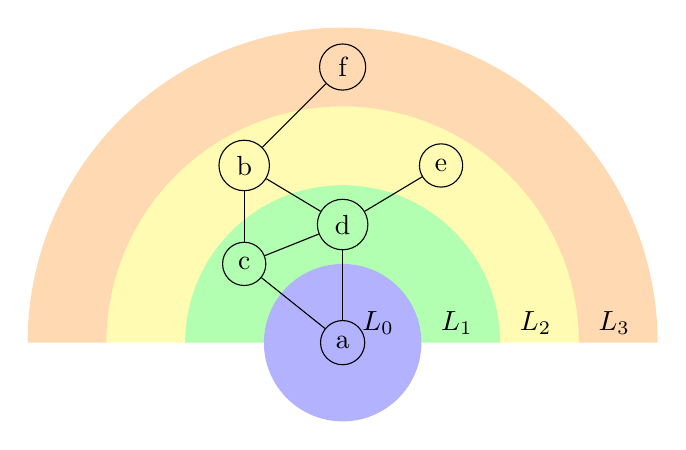
\begin{tikzpicture}[scale=0.50]
    
    \filldraw[fill=blue, fill opacity=0.3, draw=none]
    (2.5,-2) -- (2.5,0) arc (90:450:2) -- (2.5,-2);
    \filldraw[fill=green, fill opacity=0.3, draw=none]
    (4.5,-2) -- (6.5,-2) arc (0:180:4) -- (0.5,-2) arc (180:0:2);
    \filldraw[fill=yellow, fill opacity=0.3, draw=none]
    (6.5,-2) -- (8.5,-2) arc (0:180:6) -- (-1.5,-2) arc (180:0:4);
    \filldraw[fill=orange, fill opacity=0.3, draw=none]
    (8.5,-2) -- (10.5,-2) arc (0:180:8) -- (-3.5,-2) arc (180:0:6);
    
    
    \node[shape=circle,draw=black] (c) at (0,0) {c};
    \node[shape=circle,draw=black] (b) at (0,2.5) {b};
    \node[shape=circle,draw=black] (f) at (2.5,5) {f};
    \node[shape=circle,draw=black] (d) at (2.5,1) {d};
    \node[shape=circle,draw=black] (a) at (2.5,-2) {a};
    \node[shape=circle,draw=black] (e) at (5,2.5) {e} ;

    \draw (a) -- (c);
    \draw (a) -- (d);
    \draw (d) -- (c);
    \draw (d) -- (e);
    \draw (d) -- (b);
    \draw (c) -- (b);
    \draw (b) -- (f);

    \node at (3.4, -1.5) {$L_0$};
    \node at (5.4, -1.5) {$L_1$};
    \node at (7.4, -1.5) {$L_2$};
    \node at (9.4, -1.5) {$L_3$};
    
    \end{tikzpicture}

    \caption{Visualization of layers}
    \label{fig:layers}
\end{figure}

\begin{definition}[Layers]
    Given a graph $G = (V, E)$, and the vertex $a \in V$, we can define disjoint sets $L_1, L_k \subset V$ as
    \begin{equation}
        L_i = \{ b \mid \mathrm{dist}(a,b) = i \},
    \end{equation}
    where $\mathrm{dist}(a,b)$ is the distance between $a$ and $b$.
\end{definition}

By this definition, there is no edge between $i$ and $j$ if $\abs{i-j} > 1$. This fact is used to prove the generalization of Proposition \ref{prop:no-go-depth} and Theorems \ref{thm:no-go-class-i}~and~\ref{thm:no-go-class-ii} for an arbitrary connectivity constraint. The lower bound for the depth is stated in the theorem below.
\begin{proposition}
    For any arbitrary connectivity constraint $G=(V,E)$, a bridged $T$ gate where $T$ is a class I or class II gate, acting on qubits $a, b \in V$, needs at least $\mathrm{dist}(a,b) + O(1)$ depth.
\end{proposition}
\begin{proof}
  Using Lemma~\ref{lem:nontrivial-commutation}, we find $U$ defined on $a$ where the conjugation of $U$ by $T$ acts nontrivially on $b$. Now, we assume that $T = A_\ell \dots A_1$ and $u_i$ is the conjugation of $U$ by $A_i \dots A_1$. 
  
  Also, we define layers with respect to distance from $a$ as $L^{a}_i$. Now if we define trivial action on layer $L^a_i$ as the action of a gate that is trivial on every qubit in $L^a_i$, and otherwise nontrivial, now, $u_\ell$ is nontrivial on $L^a_{\mathrm{dist}(a,b)}$. The only way to make $u_\ell$ nontrivial on a layer is to apply a CNOT gate between a qubit in that layer and a qubit in another layer (assume it happens in $A_j$). Moreover, because of the fact that non-adjacent layers are not connected using edges, this CNOT must be between a qubit in $L^a_{\mathrm{dist}(a,b)}$ and a qubit in $L^a_{\mathrm{dist}(a,b) \pm 1}$. And another requirement is that $u_{j - 1}$ must be trivial on $L^a_{\mathrm{dist}(a,b) \pm 1}$. With these requirements, by a recursive argument, we can conclude that the minimum depth is $\mathrm{dist}(a,b) + O(1)$.
\end{proof}


\begin{theorem}
    For any arbitrary connectivity constraint $G=(V,E)$, a bridged $T$ gate where $T$ is a class I gate, acting on qubits $a, b \in V$, needs at least $4 \mathrm{dist}(a,b) + O(1)$ CNOTs.
\end{theorem}

\begin{proof}
    Without losing generality, we can assume $T$ is a $\mathrm{C}R_x$ with control on $a$ and target on $b$. We start by defining layers with respect to distance from $a$ as $L^{a}_i$. Then, we say a gate $U$ is acting trivially on $L^{a}_i$ if it is acting trivially on every qubit inside the set, otherwise, we say it is acting nontrivially.
    Then, noting that $b \in L^{a}_{\mathrm{dist}(a,b)}$ and non-adjacent layers are not connected using edges, we can treat these layers similarly to qubits with linear connectivity. So, by a similar argument, we can prove that $2\mathrm{dist}(a,b) + O(1)$ CNOTs are needed to make $Z_b$ defined on $b$, conjugated by $T$ act nontrivially on qubit $a$ (and trivially on qubits in layers in between) and similarly another $2\mathrm{dist}(a,b) + O(1)$ for $X_a$.
    Using the fact that layers are disjoint one can conclude these CNOTs can have $O(1)$ in common. So, the total number of CNOTs is $4\mathrm{dist}(a,b) + O(1)$.
\end{proof}

Finally, the generalised theorem for class II is written below.

\begin{theorem}
    For any arbitrary connectivity constraint $G=(V,E)$, a bridged $T$ gate where $T$ is a class II gate, acting on qubits $a, b \in V$, needs at least $6 \mathrm{dist}(a,b) + O(1)$ CNOTs.
\end{theorem}
\begin{proof}
  By defining layers with respect to distance from $a$ as $L^{a}_i$, we can treat these layers similarly to qubits with linear connectivity.
  
  Assume that there exists a CNOT between layer $L^a_0 = \{ a \}$ and $L^a_1$ that in the sequence of $T = A_\ell \dots A_1$, will take place in $A_j$.
  Then, we call the conjugation of $Z_a$ (defined on $a$) by $A^\dagger_1 \dots A^\dagger_{j-1}$ as $U_a$, that is definitely nontrivial on $L^a_0$. Lemma~\ref{lem:no-trivial-commutation} states that the conjugation of $U_a$ by $T$ (which is equal to the conjugation of $Z_a$ by $A_\ell \dots A_j$) must act nontrivial on $n$. On the other hand we know that $Z_a$ commutes with $A_j$ (which without losing generality we assumed is a CNOT with control gate in $L^a_0$). In order that $U_a$ has nontrivial action on $b$, we need to have another CNOT between these two layers. Denoting the second as $A_k$, with $j < k$, Lemma~\ref{lem:no-move-class-i} implies $U_a$ remains nontrivial on layer $2$, but undesirable for our goal, necessitating a third CNOT.
  By recursion, at least three CNOTs are needed. These arguments apply in reverse too, showing a need for $6 \cdot \mathrm{dist}(a, b) + O(1)$ CNOTs for a bridged $T$ gate between layers $a$ and $b$.
\end{proof}
  

\section{Summary of Results}

In this chapter, we have introduced a circuit for bridging class I two-qubit gates, and we have proved that this circuit is optimal in terms of CNOT count and depth. We have also proved that the baseline implementation is optimal for class II gates, in terms of CNOT count. We have also generalised these results for arbitrary connectivity constraints. The results are summarised in Table~\ref{tab:summary}.

\begin{table}[h!]
  \centering
  \begin{tabular}{c||c|c||c|c||c|c}
    \multirow{2}{*}{Class} & \multicolumn{2}{c||}{Lower bound} & \multicolumn{2}{c||}{Ours} & \multicolumn{2}{c}{Baseline} \\
    \cline{2-7}
    & CNOT & Depth & CNOT & Depth & CNOT & Depth \\
    \hline\hline
    Class I & $4n + O(1)$ & $n + O(1)$ & $4n + O(1)$ & $n + O(1)$ & $6n + O(1)$ & $3n + O(1)$ \\
    Class II & $6n + O(1)$ & $n + O(1)$ & - & - & $6n + O(1)$ & $3n + O(1)$ \\
  \end{tabular}
  \caption{Summary of results}
  \label{tab:summary}
\end{table}